\chapter{Zeemann-Effekt}
Für den Übergang von Cadmium $5^1D_2 \rightarrow 5^1P_1$ wird der normale \texttt{Zeemann}-Effekt untersucht. Dafür folgt zunächst ein theoretischer Einschub.
% -----
\section{Theoretischer Hintergrund}

Der \texttt{Zeemann}-Effekt beschreibt die Aufspaltung von Spektrallinien, und somit Aufhebung der Entartung der Energieniveaus gleicher Gesamtdrehimpulse $J$, in einem externen Magnetfeld. 
Diese Aufspaltung ist auf die Wechselwirkung des magnetischen Moments der Atome mit dem äußeren Magnetfeld zurückzuführen.
Unterschieden wird zwischen dem \textit{normalen} ($S=0$) und dem \textit{anormalen} ($S\neq 0$) \texttt{Zeemann}-Effekt.\\
Da beide Niveaus des Cd einen Gesamtspin von $S=0$ besitzen, ist nur der normale \texttt{Zeemann}-Effekt relevant.
Der Hamiltonian des Elektrons im Atom und im Magnetfeld folgt mit:
%--
\begin{equation}
    \widehat{H}= 
    \underbrace{-\frac{\hbar}{2m}\vec{\nabla}^2 
    -\frac{e^2}{4\pi\varepsilon_0 r}}_{\raisebox{1.5ex}{\scriptsize $H_\mathrm{0}$}} 
    \underbrace{+\beta\frac{\hat{\vec{L}}\cdot\hat{\vec{S}}}{\hbar^2}}_{\raisebox{1.5ex}{\scriptsize $H_{\mathrm{Spin-Bahn}}$}}
    \underbrace{+\mu_B\frac{\hat{\vec{L}}+2\hat{\vec{S}}}{\hbar}\vec{B}}_{\raisebox{1.5ex}{\scriptsize $H_{\mathrm{Zeemann}}$}}
\end{equation}
%--
mit dem \textit{Spin-Bahn}-Kopplungsterm $H_{\mathrm{Spin-Bahn}}$ aus der Feinstruktur und dem \textit{Zeemann}-Kopplungsterm $H_{\mathrm{Zeemann}}$ aus der 
Wechselwirkung mit dem äußeren Magnetfeld mit Richtung $\vec{B}=B\vec{e}_z$.\\
Da jedoch $S=0$ fallen einige Terme weg. Die guten Quantenzahlen, also die, die sich nicht ändern, sind $L$, $S$, $J$ und $M_J$ (wobei $J=L+S=L$) und die 
Energiekorrektur zum Hamiltonian ist:
%--
\begin{equation}
    \Delta E = \mu_B g_J M_J B \label{equ:energieversch}
\end{equation}
%--
mit dem Bohrschen Magneton $\mu_B = \frac{e\hbar}{2m}$ und dem Landé-Faktor $g_J$:
%--
\begin{equation}
    g_J = 1 + \frac{J(J+1) + S(S+1) - L(L+1)}{2J(J+1)}
\end{equation}
%--
Die Aufspaltung der Energieniveaus und möglichen Übergänge für die verschiedenen $M_J$ anhand der Auswahlregeln
%--
\begin{align*}
    \Delta J &= 0, \pm 1\\
    \Delta M_J &= 0, \pm 1
\end{align*}
%--
sind in \cref{fig:cd_niveaus} dargestellt.
%--
%\clearpage
Die Polarisation der Strahlung hängt von der Änderung der magnetischen Quantenzahl $M_J$ im Übergang ab (siehe \cref{fig:polarisation}):
%--
\begin{itemize}
    \item \textbf{$\pi$-Übergänge:} $\Delta M_J = 0$ — linear polarisiert parallel zur Magnetfeldrichtung
    \item \textbf{$\sigma^+$-Übergänge:} $\Delta M_J = +1$ — rechtszirkular polarisiert (bei longitudinaler Beobachtung)
    \item \textbf{$\sigma^-$-Übergänge:} $\Delta M_J = -1$ — linkszirkular polarisiert (bei longitudinaler Beobachtung)
\end{itemize}
%--
Je nach Beobachtungsrichtung relativ zum Magnetfeld lassen sich unterschiedliche Polarisationen der emittierten Strahlung beobachten:
%--
\begin{itemize}
    \item \textbf{Longitudinale Konfiguration:} Magnetfeld $B$ ist parallel zur Beobachtungsrichtung. Es treten ausschließlich zirkular polarisierte Anteile auf ($\sigma^+$ und $\sigma^-$).
    \item \textbf{Transversale Konfiguration:} Magnetfeld $B$ ist senkrecht zur Beobachtungsrichtung. Es treten linear polarisierte Komponenten auf ($\pi$- und $\sigma$-Komponenten).
\end{itemize}
%--
\begin{figure}[ht]
    \centering
    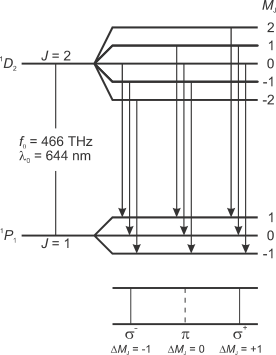
\includegraphics[width=.4\linewidth]{Niveauaufspaltung_Cd.png}
    \caption[Niveauaufspaltung des$5^1D_2 \rightarrow 5^1P_1$-Übergangs bei Cd]{Niveauaufspaltung des $5^1D_2 \rightarrow 5^1P_1$-Übergangs beim normalen \texttt{Zeemann}-Effekt an Cadmium~\cite{LD}}\label{fig:cd_niveaus}
\end{figure}
%--
\begin{figure}[!ht]
    \centering
    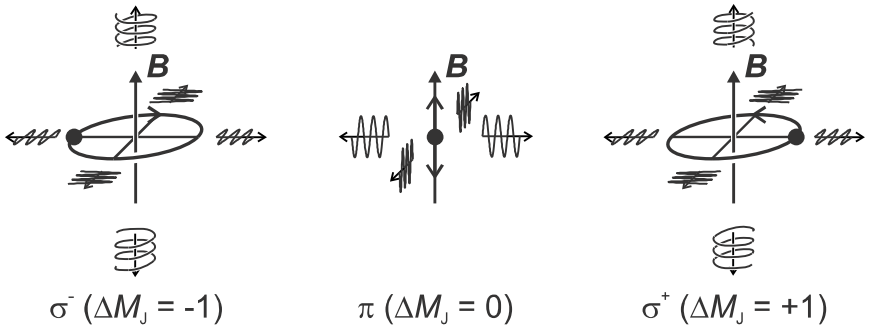
\includegraphics[width=.55\linewidth]{Dipolstrahlung_Verteilung.PNG}
    \caption[Winkelverteilung der elektischen Dipolstrahlung]{Winkelverteilung der elektischen Dipolstrahlung; $\Delta M_J$ -- Drehimpulsrichtung der emittierten Photonen~\cite{LD}}\label{fig:polarisation} % chktex 8
\end{figure}
%
% -----
%
%\clearpage
\section{Aufbau}
Zur Untersuchung des \texttt{Zeemann}-Effekts wird eine Cadmiumlampe verwendet, deren Emissionsspektrum die relevante rote Spektrallinie bei $\lambda = 644 \, \mathrm{nm}$ enthält. Die Lampe befindet sich zwischen den Polschuhen eines Elektromagneten, dessen homogenes Magnetfeld durch ein Hochstromnetzgerät erzeugt und über eine Hall-Sonde kallibriert wird. Die optische Strahlführung umfasst folgende Komponenten zu Erzeugung eines Interferenzbildes (siehe \cref{fig:aufbau_zeemann}):
%--
\begin{itemize}
    \item Eine \textbf{Kondensorlinse} (Brennweite $f = \SI{150}{\milli\meter}$ erzeugt eine parallele Beleuchtung).
    \item Ein \textbf{Fabry-Pérot-Etalon} mit einem Plattenabstand von $d = \SI{4}{\milli\meter}$, einem Brechungsindex $n = 1.457$ und einem Reflexionsgrad von $R = 0.85$.
    \item Eine Abbildungslinse (ebenfalls $f = \SI{150}{\milli\meter}$) bildet die Interferenzringe ab.
    \item Ein \textbf{Interferenzfilter} mit einer Mittelwellenlänge von $\lambda = \SI{643,8\pm 2,0}{\nano\meter}$ selektiert die zu untersuchende Spektrallinie.
    \item Zur Analyse der Polarisation werden ein Polarisationsfilter und eine Viertelwellenlängeplatte verwendet.
\end{itemize}
%--
\begin{figure}[ht]
    \centering
    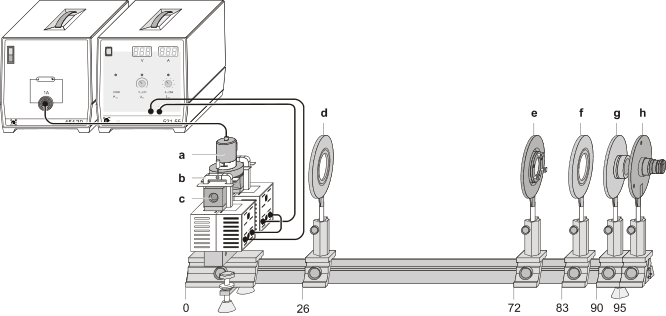
\includegraphics[width=.7\linewidth]{ZeemanAufbau.png}
    \caption[Aufbau der Versuchsanordnung zum Zeemann-Effekt]{Versuchsaufbau zur Messung des \texttt{Zeemann}-Effekts mit (a) Cadmiumlampe, (b) Klammern, (c) Polschuhe, (d) / (f) Sammellinsen, (e) Fabry-Pérot-Etalon, (g) Interferenzfilter und (h) Okular mit Strichskala~\cite{LD}.}\label{fig:aufbau_zeemann}
\end{figure}
%--
Die Beobachtung erfolgt zunächst mit einem Okular. Für die quantitative Auswertung wird das Okular dann durch eine CCD-Kamera ersetzt, welche das Intensitätsprofil der Interferenzringe entlang einer Linie in das Messprogramm überträgt.
\vspace{0.3cm}\\
Das \texttt{Fabry-Pérot}-Etalon (\cref{fig:fabry_perot}) ist ein Interferometer, das zur hochauflösung spektraler Aufspaltung genutzt wird. Es besteht aus zwei planparallelen, hochreflektierenden Glasplatten mit einem festen Abstand $d$ zueinander. Licht, dass in einem bestimmten Winkel $\alpha$ in das Etalon eintritt, wird an den beiden Platten mehrfach hin- und herreflektiert, sodass durch Interferenz bestimmte Wellenlängen konstruktiv verstärkt und andere ausgelöscht werden.
%--
\begin{figure}[ht]
    \centering
    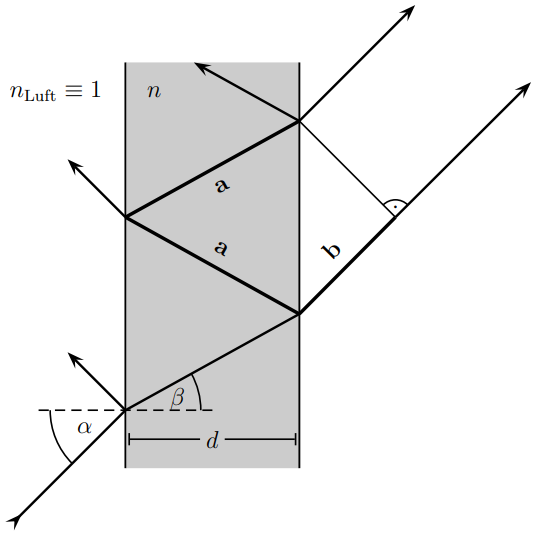
\includegraphics[width=.4\linewidth]{Fabry_Perot.PNG}
    \caption[Fabry-Pérot-Etalon]{Intensität der Interferenzringe in Abhängigkeit von der Wellenlänge~\cite{LD}.}\label{fig:fabry_perot}
\end{figure}
%--

\noindent Die Bedingung für konstruktive Interferenz ergibt sich aus dem optischen Wegunterschied zwischen den reflektierten Teilstrahlen:
%--
\begin{equation}
    2nd \cos(\alpha) = m \lambda \label{equ:fabry_perot}
\end{equation}
%--
wobei $n$ der Brechungsindex des Mediums zwischen den Platten, $d$ der Abstand der Platten, $m \in \mathbb{Z}$ die Interferenzrdnung und $\lambda$ die Wellenlänge des Lichts ist.\\
Die resultierende Intensitätsverteilung zeigt sich in Form konzentischer Ringe (Interferenzringe), die bei Verwendung eines monochromatischen Lichtfilters einer bestimmten Spektrallinie zugeordnet werden können.\\
Die Finesse $\mathcal{F}$ des Etalons beschreibt die Güte der Interferenz und ist definiert als das Verhältnis der Wellenlängenabstände $\Delta \lambda$ der benachbarten Maxima zur Breite $\Delta \lambda_0$ des zentralen Maximums:
%--
\begin{equation}
    \mathcal{F} = \frac{\Delta \lambda}{\Delta \lambda_0} = \frac{\pi\sqrt{R}}{1-R}
\end{equation}
%--
Die Finesse  ist ein Maß für die Anzahl der Interferenzmaxima, die innerhalb einer bestimmten Wellenlängenbreite auftreten können.\\
Die Auflösung $A$ des Etalons ist definiert als das Verhältnis der Wellenlängen $\lambda$ zur Breite $\Delta \lambda$ der Maxima:
%--
\begin{equation}
    A = \frac{\lambda}{\Delta \lambda}
\end{equation}
%--
Die Auflösung ist ein Maß dafür, wie gut das Etalon in der Lage ist, benachbarte Spektrallinien zu trennen.\\
%
%--
%
\section{Beobachtung der Aufspaltung}
%
%--
%
\subsection{Justage}
Nachdem die Lampe für etwa 2 Minuten warm gelaufen ist, wird der optische Aufbau mit Hilfe des Okulars justiert, um ein symmetrisches und zentriertes Interferenzmuster zu erhalten.\\
Dafür wird zunächst das Okular scharf auf die Strichskala eingestellt. Die Cadmiumlampe wird so positioniert, dass die Lichtquelle möglichst mittig im Magnetfeld liegt. Die Kondensorlinse wurde justiert, um eine parallele Ausleuchtung des Etalons zu erreichen.\\
Die Position der zweiten Linse sowie des Beobachtungspfades (jetzt Okular später CCD-Kamera) werden so eingestellt, dass das durch das Fabry-Pérot-Etalon erzeugte Ringsystem mittig und scharf abgebildet wird.\\
Durch leichtes Kippen des Etalons kann das Zentrum des Ringsystems auf die Strichskala eingestellt werden.
\vspace{0.3cm}\\
Um longitudinale und transversale Konfigurationen zu untersuchen wird die Halterung der Spulen zusammen mit der Cd-Lampe um $90^{\circ}$ gedreht (\cref{fig:aufbau_zeemann_above}).\\
%--
\begin{figure}[H]
    \centering
    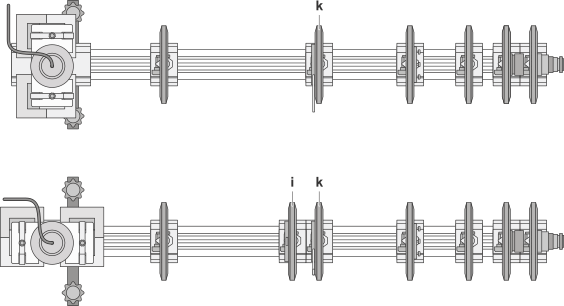
\includegraphics[width=.6\linewidth]{ZeemanAufbaufromAbove.png}
    \caption[Longitudinale und Transversale Konfiguration Zeemann-Effekt]{Aufbau zur Messung in transversaler Konfiguration (oben) und longitudinaler Konfiguration (unten) von oben betrachtet mit (i) Viertel-Wellenlängen-Platte und (k) Polarisationsfilter~\cite{LD}.}\label{fig:aufbau_zeemann_above}
\end{figure}
%--
\noindent Zur Beobachtung der jeweiligen Komponenten werden die Polarisationsfilter und die Viertelwellenlängenplatte in den Strahlengang eingebaut.
%
%--
%
\subsection{Transversale Konfiguration}
%--
\begin{figure}[ht]
    \centering
    \subcaptionbox{\texttt{Zeemann}-Aufspaltung in transversaler Konfiguration (A) ohne Magnetfeld, (B) mit Magnetfeld, (C) mit Polarisationsfilter auf $0^{\circ}$ und (D) mit Polarisationsfilter auf $90^{\circ}$. Für das Magnetfeld wurde der Strom jeweils auf $\SI{6,9}{\ampere}$ eingestellt\label{fig:trans_all}}{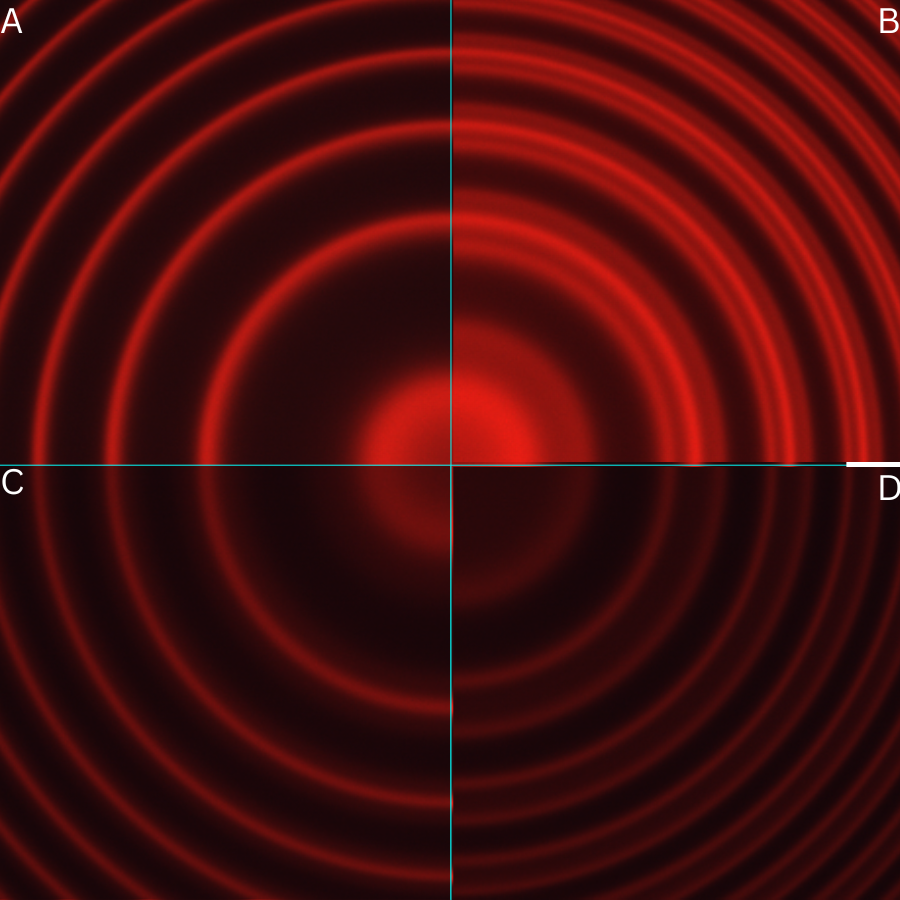
\includegraphics[width=0.45\textwidth]{Transversal.png}}
    \subcaptionbox{Einstellung des Stroms auf $\SI{4,7}{\ampere}$ bis die aufgespalteten Linien ohne Filter gerade unterschieden werden können\label{fig:trans_strom}}{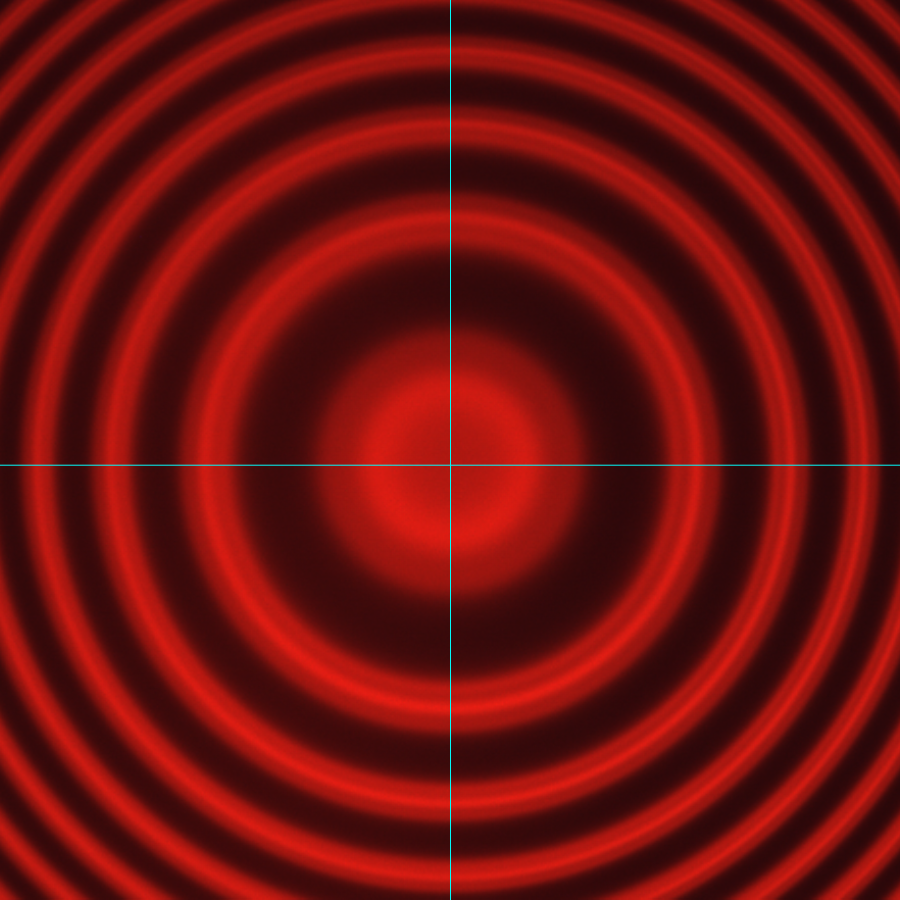
\includegraphics[width=0.45\textwidth]{Trans_Strom.png}}
    \caption{Beobachteter \texttt{Zeemann}-Effekt in transversaler Konfiguration.}
\end{figure}
%--
\clearpage
\noindent Bei Ausgeschaltetem Magnetfeld (\cref{fig:trans_all} (A)) sind die konzentrischen Interferenzringe durch Mehrfachinterferenz von kohärentem Licht im Etalon sichtbar. Die verwendetete Cd-Lampe emmitiert spektrale Linien, unter anderem bei einer Wellenlänge von $\lambda = \SI{643,8}{\nano\meter}$, die einem elektronischen Übergang vom angeregten Zustand $5^1D_2$ in den Grundzustand $5^1P_1$ entspricht. Um sicherzustellen, dass ausschließlich diese Übergangslinie beobachtet wird, wird durch den Interferenzfilter eine Durchlassbreite von $\pm \SI{2}{\nano\meter}$ ausgewählt.
\vspace{0.2cm}\\
Der Magnetstrom wird auf $\SI{6,9}{\ampere}$ eingestellt, sodass die Aufspaltung der Spektrallinie sichtbar wird (\cref{fig:trans_all} (B)). Der mittlere Ring ist dabei am stärksten ausgeprägt und entspricht der $\pi$-Komponente ($\Delta M_J=0$), während die äußeren Ringe innen schwächer sind und den $\sigma^\pm$-Komponenten ($\Delta M_J=\pm 1$) entsprechen.\\ 
Die $\sigma$-Komponenten werden über ihre radiale Verschiebung im Interferenzbild identifiziert: Die Linie mit geringerer Wellenlänge ($\sigma^+$) ist nach außen verschoben, die Linie mit größerer Wellenlänge ($\sigma^-$) nach innen.\\
Die intensität der Komponenten variiert im Verlauf der Messung, insbesondere im Vergleich zum Bild ohne Magnetfeld.
\vspace{0.2cm}\\
\noindent Bei Verwendung des Polarisationsfilters auf $0^{\circ}$ (\cref{fig:trans_all} (C)) zwischen Kondensonrlinse und Etalon werden die $\sigma^\pm$-Komponenten aufgrund ihrer Polarisationsrichtung herausgefiltert.
\vspace{0.2cm}\\
\noindent Wird der Polarisationsfilters nun auf $90^{\circ}$ eingestellt (\cref{fig:trans_all} (D)), wird die $\pi$-Komponente herausgefiltert, sodass nur die $\sigma^\pm$-Komponenten sichtbar sind.
%
%--
%
\subsection{Longitudinale Konfiguration}
%--
\begin{figure}[ht]
    \centering
    \subcaptionbox{\texttt{Zeemann}-Aufspaltung in longitudinaler Konfiguration (A) ohne Magnetfeld, (B) mit Magnetfeld, (C) mit Viertel-Wellenlänge-Platte auf $0^{\circ}$ und Polarisationsfilter auf $-45^{\circ}$ und (D) mit Viertel-Wellenlänge-Platte auf $0^{\circ}$ und mit Polarisationsfilter auf $+45^{\circ}$. Für das Magnetfeld wurde der Strom jeweils auf $\SI{2,5}{\ampere}$ eingestellt\label{fig:long_all}}{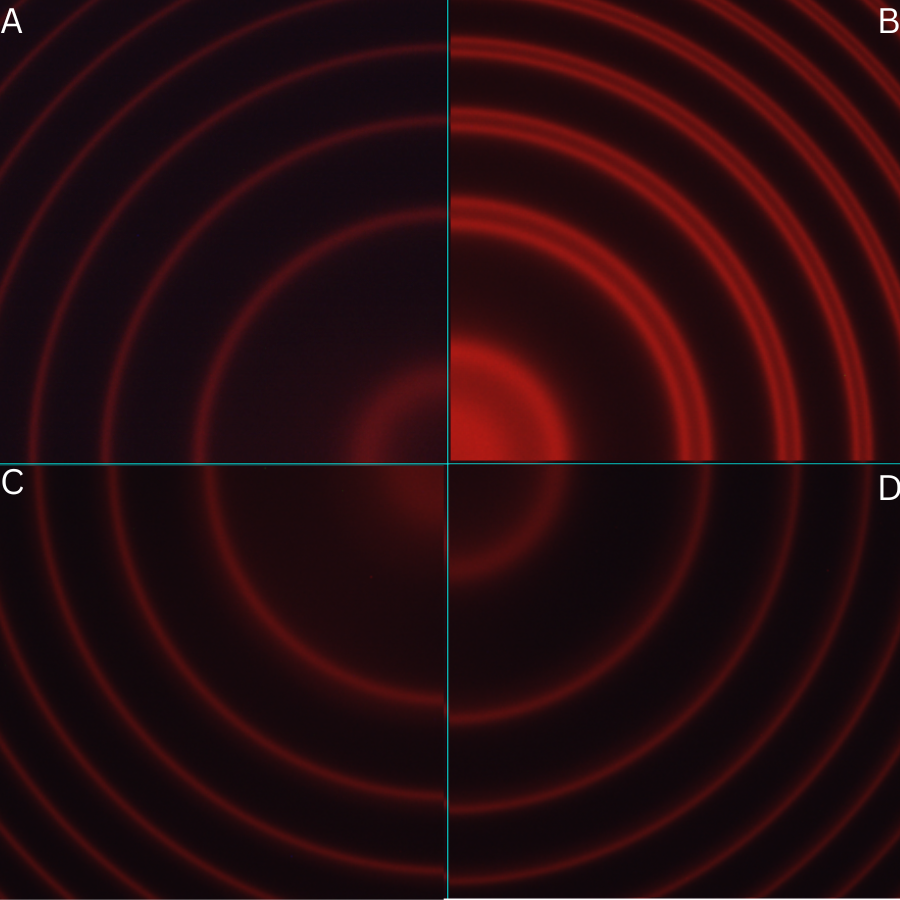
\includegraphics[width=0.45\textwidth]{Longitudinal.png}}
    \subcaptionbox{Einstellung des Stroms auf $\SI{1,7}{\ampere}$ bis die aufgespalteten Linien ohne Filter gerade unterschieden werden können\label{fig:long_strom}}{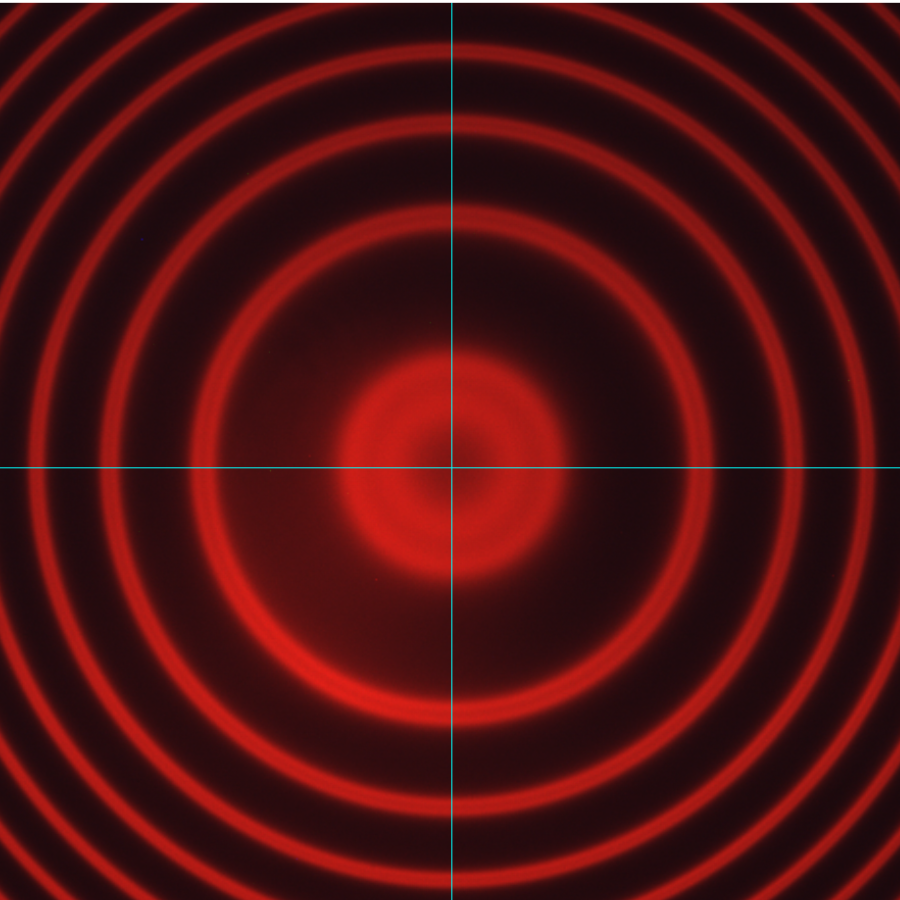
\includegraphics[width=0.45\textwidth]{Long_Strom.png}}
    \caption{Beobachteter \texttt{Zeemann}-Effekt in longitudinaler Konfiguration.}
\end{figure}
%--
\noindent Bei ausgeschaltetem Magnetfeld (\cref{fig:long_all} (A)) sind wieder die konzentrischen Interferenzringe sichtbar.
\vspace{0.2cm}\\
\noindent Erhöht man nun den Magnetstrom auf $\SI{2,5}{\ampere}$ (\cref{fig:long_all} (B)), so erfolgt eine Aufspaltung der Spektrallinie in die $\sigma^\pm$-Komponenten, die sich radial verschieben. Bei dieser Konfiguration ist die $\pi$-Komponente nicht sichtbar, da sie in der Richtung des Magnetfeldes polarisiert ist.
\vspace{0.2cm}\\
\noindent Bei Verwendung der Viertelwellenlängenplatte auf $0^{\circ}$, welche das zirkular polarisierte Licht in linear polarisiertes Licht umwandelt, und des Polarisationsfilters auf $-45^{\circ}$ (\cref{fig:long_all} (C)) werden die $\sigma^+$-Komponente sichtbar und die $\sigma^-$-Komponente herausgefiltert. Dies erfolgt, indem durch die Viertelwellenlängenplatte der zur Plattenachse parallel polarisierten Anteil der $\sigma^+$-Komponente um $90^{\circ}$ gedreht wird.
\vspace{0.2cm}\\
\noindent Wird der Polarisationsfilter nun auf $+45^{\circ}$ eingestellt (\cref{fig:long_all} (D)), so wird die $\sigma^-$-Komponente sichtbar und die $\sigma^+$-Komponente herausgefiltert.\\
\newpage
\section{Messung der Aufspaltung}
%--
Um die betrachtete Aufspaltung quantitativ zu untersuchen, wird das Okular durch eine \texttt{CCD}-Kamera ersetzt und mit einer \texttt{Hall}-Sonde die magnetische Feldstärke gemessen.
%
%--
%
\subsection{Kalibrierung des Magnetfeldes}\label{sec:kal_magnetfled}
%--
Vor und nach der Messung wird die Abhängigkeit der magn. Feldstärke vom durch die Spulen fließenden Strom bestimmt. Hierfür wird eine \texttt{Hall}-Sonde auf einem optischen Reiter befestigt und mittig zwischen den Polschuhen anstelle der Cd-Lampe platziert. Dann wird die Messung gestartet und in regelmäßigen Abständen der Strom erhöht (bis $I_{\text{max}}\approx \SI{10}{\ampere}$). Die Messfehler folgen aus~\cite{LD} mit $\Delta I = \SI{1.5}{\percent}$ für den Strom und $\Delta B = \SI{2}{\percent} + \SI{0.5}{\percent}\cdot B_{\text{max}}$ wobei $B_{\text{max}}$ der Bereichsendwert ist.\\
Zur Modellierung der Daten wird ein Polynome 3. Grades\footnote{Polynome 2. Grades reichen meist um leichte Nichtlinearitäten zu modellieren, jedoch kann ein weiterer Grad hilfreich sein, um mögliche Sättigung des Eisenkerns und damit Abflachung der Stromkurve zu berücksichtigen} verwendet, um bei gegebenem Spulenstrom die magn. Flussdichte zu berechnen:
\begin{equation*}
    f(x) = ax^3 + bx^2+xc+d
\end{equation*}
Dieses wird nun mit Hilfe von \texttt{curve\_fit} an die Datensätze angepasst (\cref{fig:magnetfeldkali_ges}). Die Kalibration erfolgt durch Mitteln der Anpassungsfunktionen zu einer \textit{Gesamtanpassungs}kurve.
\begin{figure}[h]
    \centering
    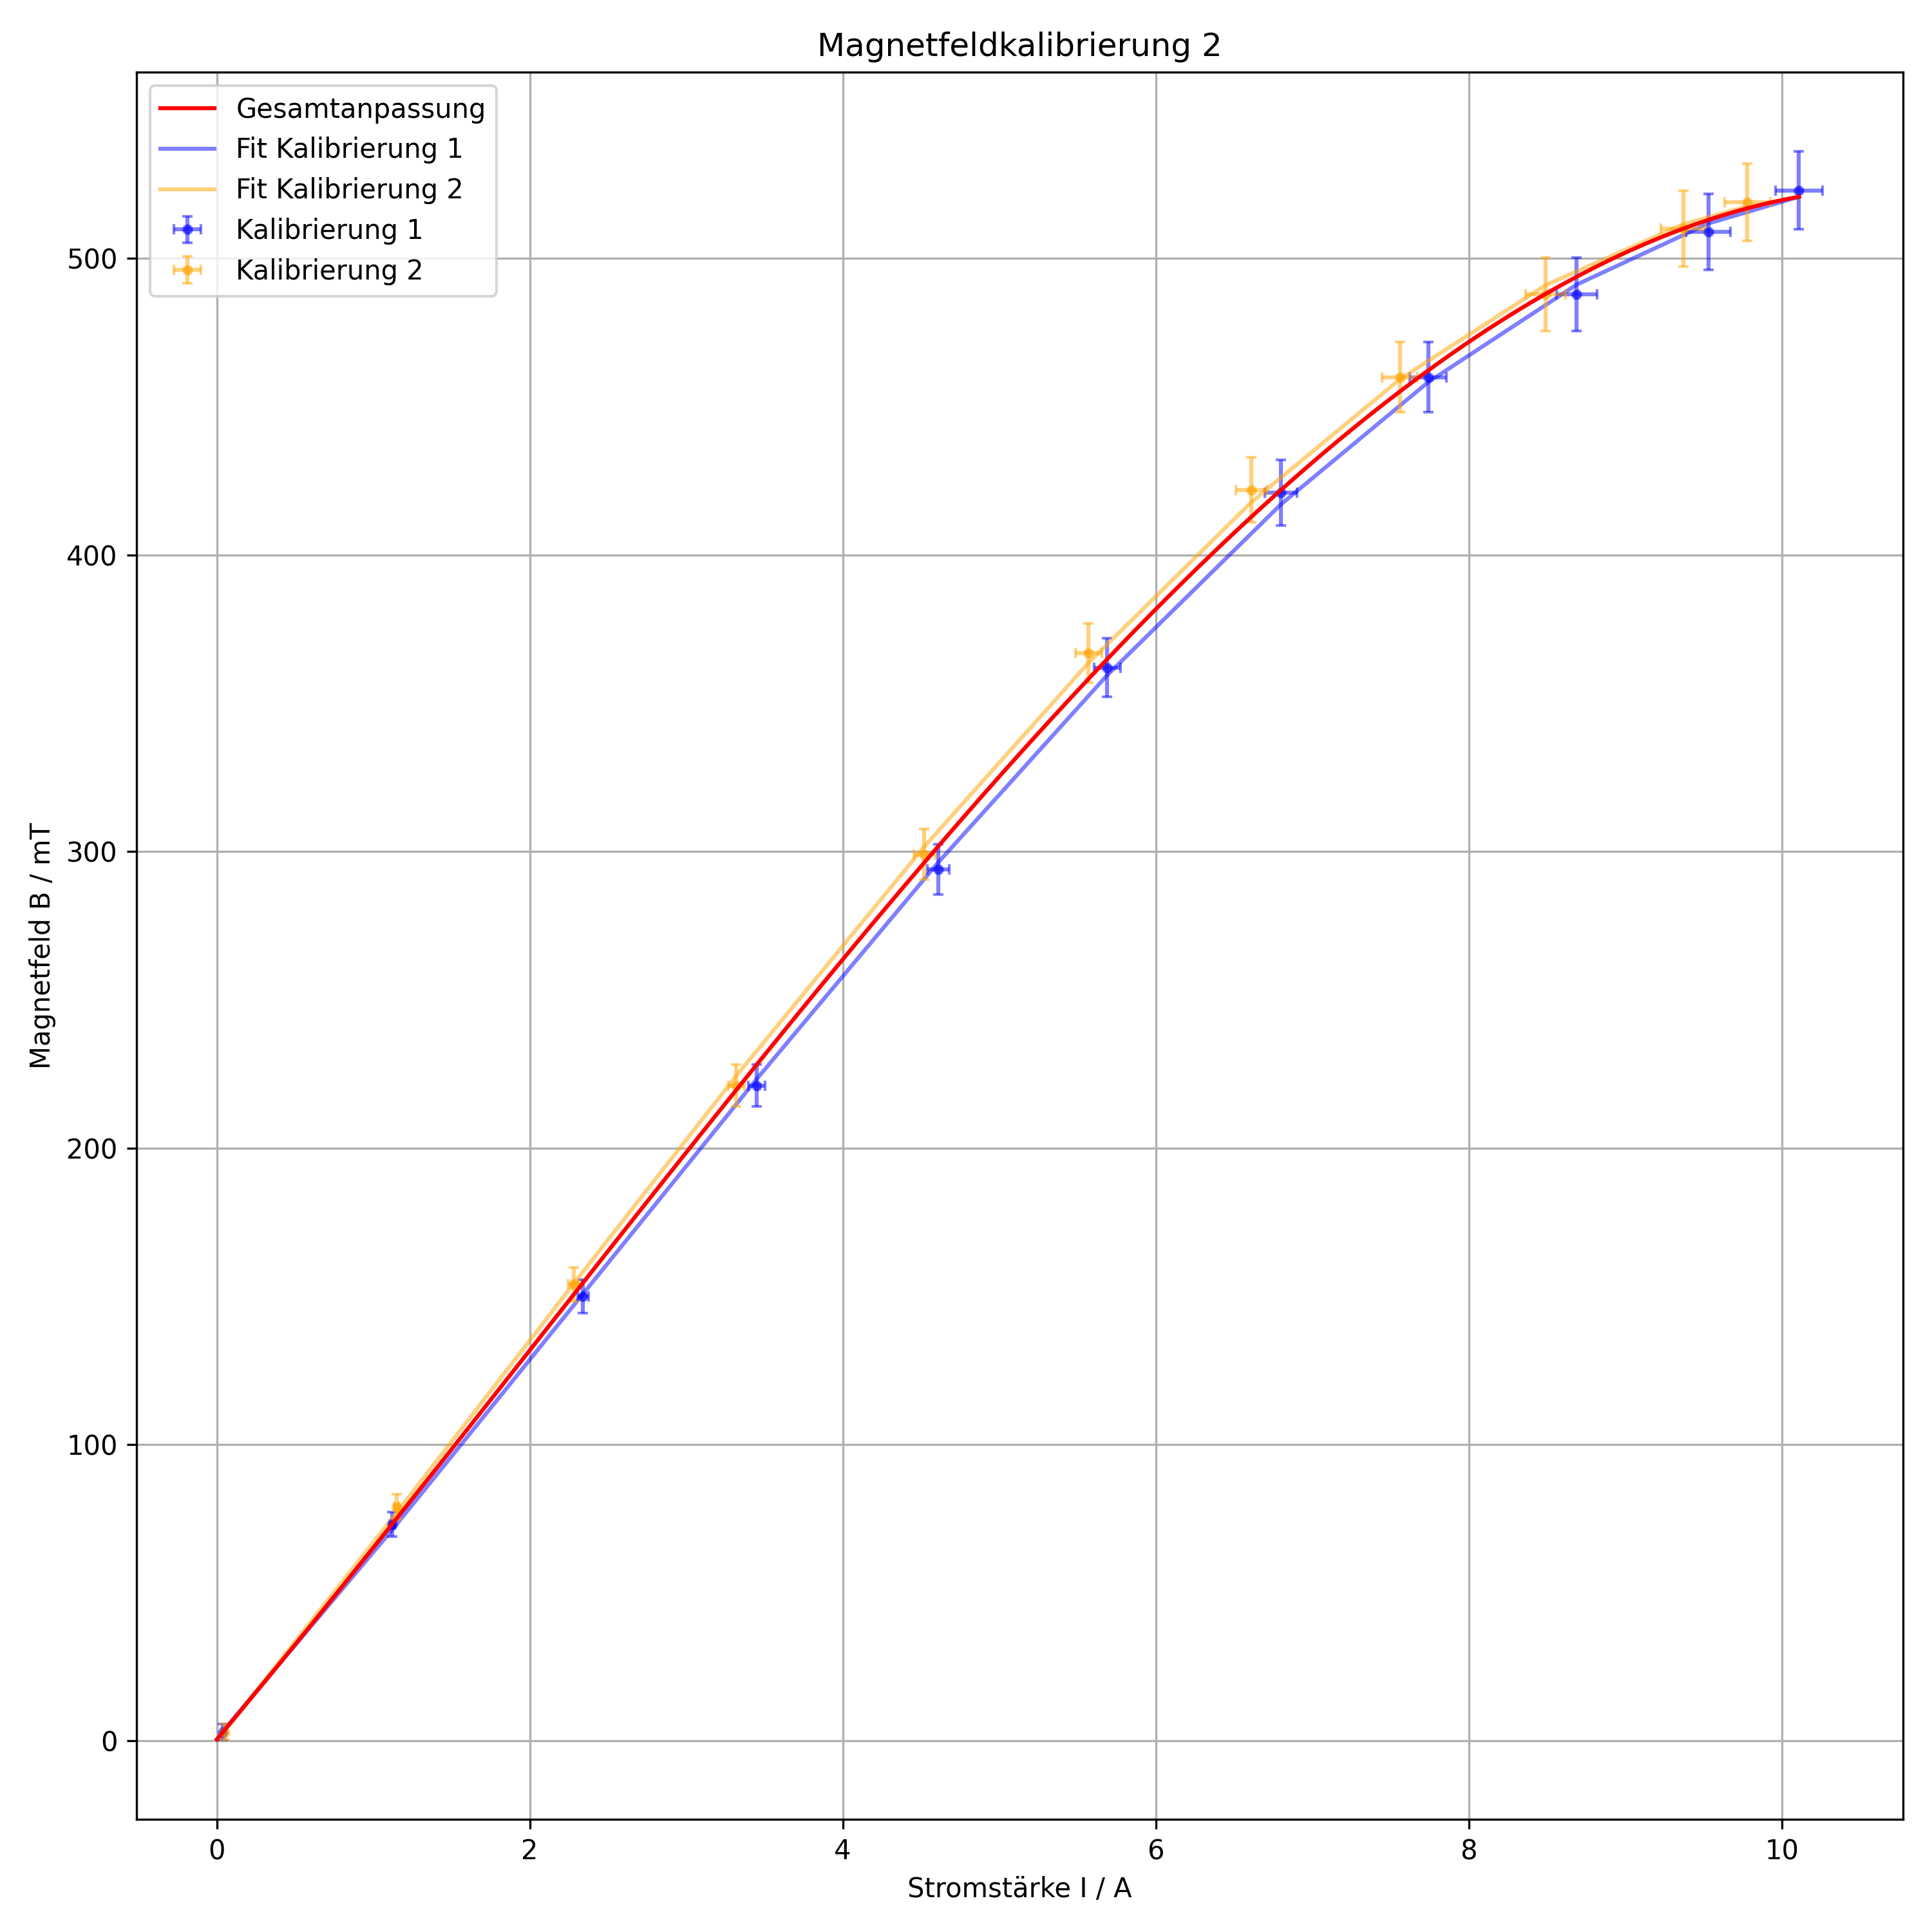
\includegraphics[width=0.8\linewidth]{plots/zeeman_pltKalibrierung_gesamt.png}
    \caption{Messdaten der magnetische Flussdichte $B$ gegen den Spulenstrom $I$ mit einer Anpassungsfunktion $ f(x)=ax^3+bx^2+cx+d $. Die Gesamtanpassung erfolgt durch Mitteln beider Anpassungskurven.}\label{fig:magnetfeldkali_ges}
\end{figure}
\begin{table}[h!]
    \centering
    \begin{tabular}{
        l|
        S[table-format=2.3(3)]
        S[table-format=1.3(4)]
        S[table-format=2.3(4)]
        S[table-format=1.3(4)]
    }
    \toprule
    \multicolumn{1}{l|}{} & 
    \multicolumn{1}{c}{$a$ [T]} & 
    \multicolumn{1}{c}{$b$ [T/A]} & 
    \multicolumn{1}{c}{$c$ [T/A$^2$]} & 
    \multicolumn{1}{c}{$d$ [T/A$^3$]} \\
    \midrule
    Kalibrierung 1 & -0.298 \pm 0.094 & 2.09 \pm 1.27 & 60.78 \pm 4.21 & 0.93 \pm 2.70 \\
    Kalibrierung 2 & -0.297 \pm 0.102 & 1.62 \pm 1.35 & 65.45 \pm 4.36 & 0.10 \pm 2.74 \\
    \midrule
    Gesamtanpassung & -0.297 \pm 0.098 & 1.86 \pm 1.31 & 63.11 \pm 4.29 & 0.51 \pm 2.72 \\
    \bottomrule
    \end{tabular}
    \caption{Anpassungsparameter der Magnetfeld-Kalibrierungen}\label{tab:kalibrierung}
\end{table}
Man erkennt, dass die Messpunkte der zweiten Kalibrierungskurve etwas höher liegen, jedoch unterscheiden sich beide Messpunkte insgesamt nur sehr leicht und ihre Fehlerbalken überlappen.\footnote{Kleinere Schwankungen zwischen den Messungen sind durch leicht verschobene Positionen der \texttt{Hall}-Sonde zu erklären}
%
%--
%
\newpage
\subsection{Bestimmung der Peakschwerpunkte}
%--
Die \texttt{Hall}-Sonde wird nun aus dem Aufbau entfernt und die Cd-Lampe wieder eingesetzt.\\
Gemessen wird die Intensität der Interferenzringe entlang einer Achse (als Pixelkoordinate).
Diese Pixelkoordinate wird zum späteren Auftragen zunächst in einen Winkel $\alpha$ umgeformt mit:
%--
\begin{equation*}
    \alpha = \frac{\Delta p \cdot s}{f}
\end{equation*}
%--
wobei $\Delta p$ den Abstand zwischen zwei Ringen (in Pixel), $s=\SI{9.6e-6}{\meter}$ die Pixelgröße und $f=\SI{150}{\milli\meter}$ Die Brennweite der Abbildungslinse entsprechen.\\
Die Abbildungslinse ist so einzustellen, dass die Peaks der beobachteten Kurve scharf sind und die maximale Intensität haben. Dann wird das Etalon so gekippt, bis das Zentrum des Ringsystems auf die CCD-Zeile abgebildet wird, keine weiteren Peaks mehr hervorquellen und der Mittelpunkt der ersten beiden Peaks mittig auf der Messkala ist.\\
Zunächst erfolgt eine Messung ohne Magnetfeld, anschließend jeweils eine Messung ab $I=\SI{1.0}{\ampere}$ in $\SI{1.0}{\ampere}$-Schritten bis $I_{\text{max}}=\SI{10,0}{\ampere}$\\
Beispielhaft werden im folgenden die Messungen für $I = \SI{10,0}{\ampere}$ aufgeführt (\cref{fig:messung_10A} und \cref{fig:peak_10A}), wobei eine aufgespaltene Linie für die Auswertung genauer betrachtet wird. Hierfür wurde die dem Zentrum zur linken nächsten Linie im Bereich $\alpha \in \left[\SI{1.5}{\degree}\; ,\;\SI{1.8}{\degree}\right]$ gewählt.
%--
\begin{figure}[ht]
    \subcaptionbox{Messung der \texttt{CCD}-Kamera für einen Strom von \\$I = \SI{10,0}{\ampere}$. Zur besseren Verdeutlichung wurden die Messpunkte zusätzlich miteinander verbunden.\label{fig:messung_10A}}{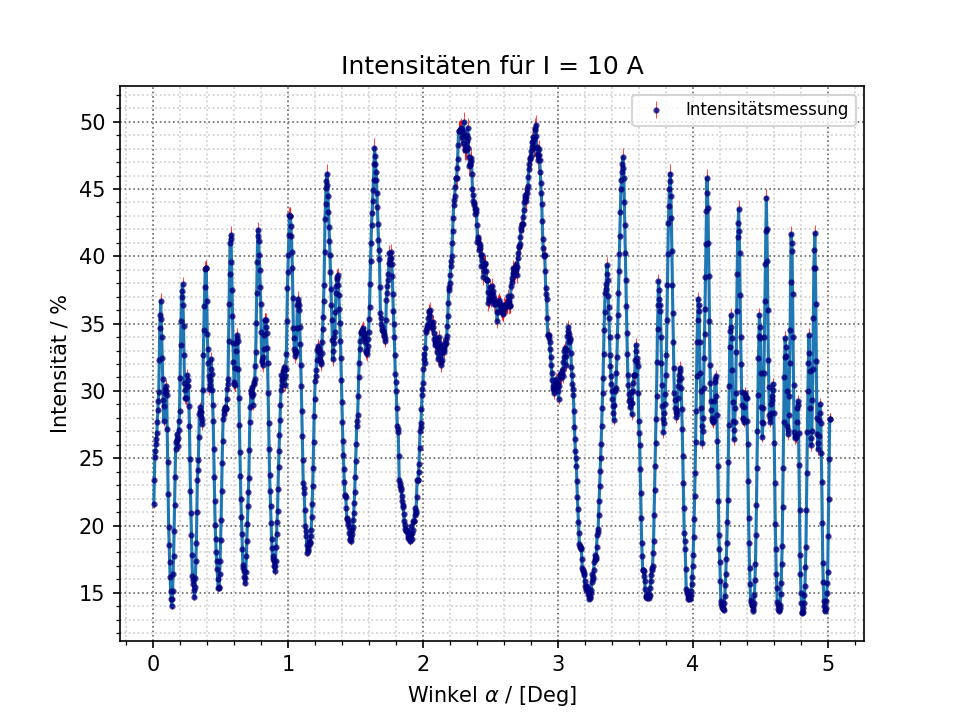
\includegraphics[width=.5\textwidth]{plots/ZeemanX_10A.png}}
    %\subcaptionbox{Messung der \texttt{CCD}-Kamera ohne Magnetfeld. Zur besseren Verdeutlichung wurden die Messpunkte zusätzlich miteinander verbunden.}{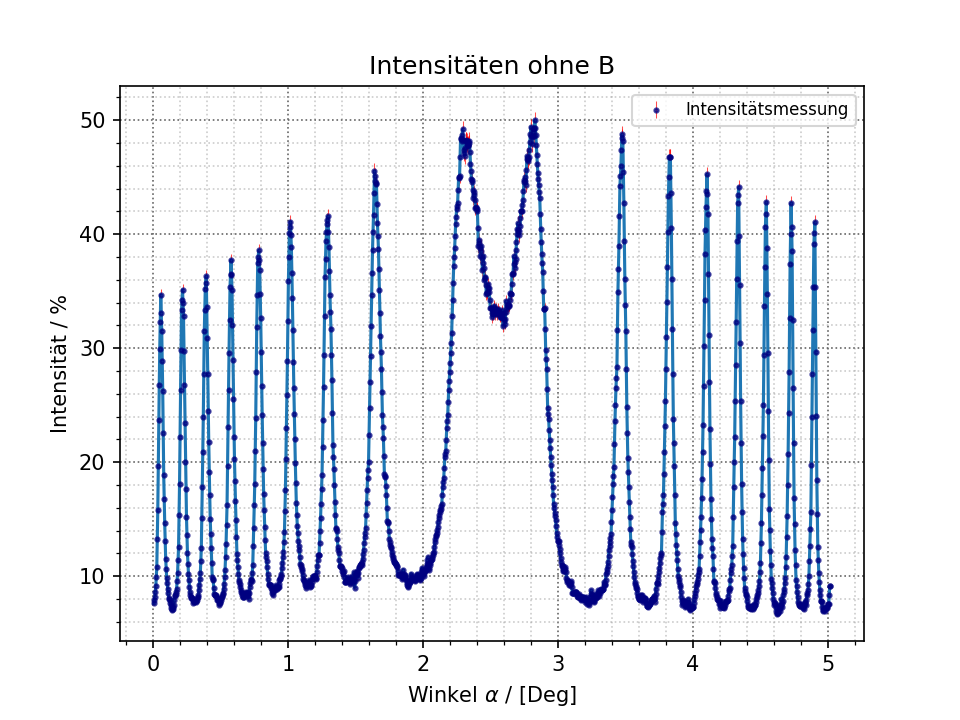
\includegraphics[width=.5\textwidth]{plots/ZeemanX_ohne_B.png}}
    \subcaptionbox{Vergrößerte der \texttt{CCD}-Kamera für einen Strom von \\$I = \SI{10,0}{\ampere}$. \label{fig:peak_10A}}{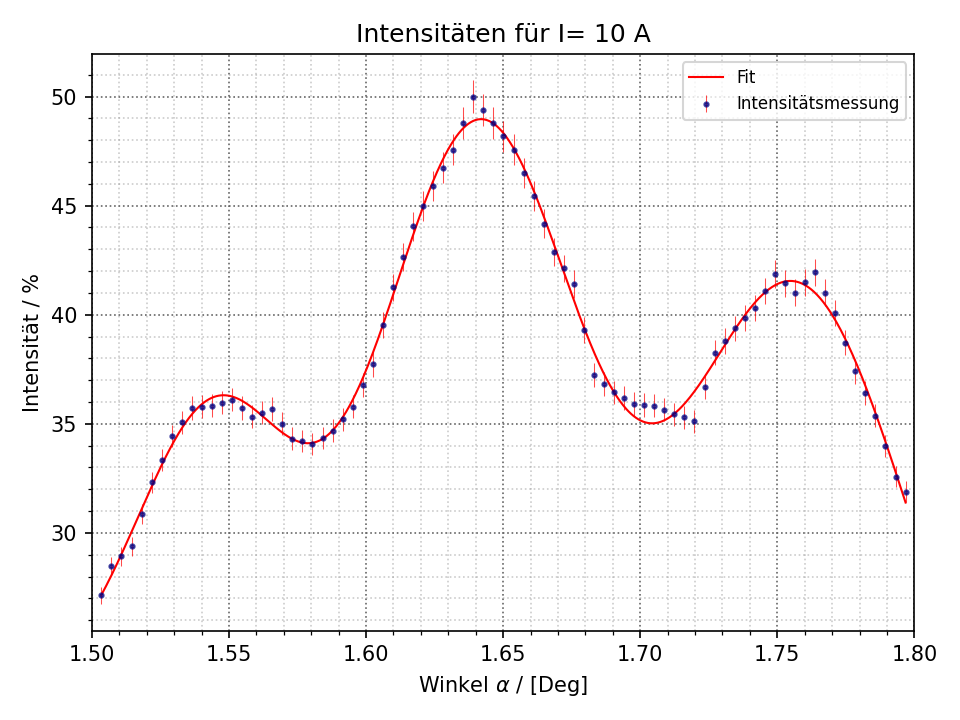
\includegraphics[width=.5\textwidth]{plots/peak_10A.png}}
\end{figure}
%--

\noindent Das Signal kann durch eine Summe dreier \texttt{Gauss}-Funktionen modelliert werden. Zusätzlich wird eine lineare Funktion zur Modellierung der nach außen abfallenden Intensität verwendet, sodass folgt:
\begin{equation*}
    f(x) = a + bx + \sum^{3}_{i=1} \frac{A_i}{\sigma_i\sqrt{2\pi}}\exp{-\frac{(x-\mu_i)^2}{2\sigma_i^2}}
\end{equation*}
\newpage
Dies wird mit Hilfe des Python-Pakets \texttt{lmfit} an die Daten für alle 10 Aufnahmen bei verschiedenen Spulenströmen durchgeführt.\footnote{Hier sollte zunächst der Strom langsam erhöht werden bis die Spektrallinien voneinander getrennt sind, um einen sinnvollen Messbereich wählen zu können (ab dem Start der Aufspaltung in 10 Intervallschritten). Dies wurde falsch verstanden, weswegen die ersten Messwerte keine Aufspaltung der Spektrallinien aufzeigen (erst sichtbar bei einem Strom von $I=\SI{5,6}{\ampere}$). Im weiteren Verlauf der Auswertung werden nur die Messwerte mit einem Strom ab $I = \SI{6}{\ampere}$ verwendet.}
Die Ergebnisse dieser Anpassung sind in \cref{tab:langzeeman-fit} einzusehen. Die Anpassungsgüten $\chi_{\text{red}}^2$ liegen zwischen $0,67$ und $0,86$ was für eine akzeptable Anpassung spricht. Dies kann man auch in \crefrange{fig:peaks_all_a}{fig:peaks_all_b} erkennen.\\
Die Peakschwerpunkte $\mu_i$ ($i = \{1,2,3\}$) entsprechen den Beugungswinkeln für die verschiedenen Linien und werden wie folgt definiert:
\begin{align*}
    \mu_1 &= \alpha_{\sigma^-}, & \mu_2 &= \alpha_{\pi}, & \mu_3 &= \alpha_{\sigma^+}
\end{align*} 
Die Spulenströme werden mit Hilfe der Magnetfeldkalibrierung in magnetische Flussdichten umgerechnet (\cref{tab:spulenstroeme})
\begin{table}[h!]
    \centering
    \begin{tabular}{
        S[table-format=1]
        S[table-format=2.3(3)]
        S[table-format=1.3(4)]
    }
    \toprule
    \multicolumn{1}{c}{Messungs-Nr.} & 
    \multicolumn{1}{c}{Spulenstrom [A]} & 
    \multicolumn{1}{c}{Magn. Flussdichte [T]} \\
    \midrule
    1 & 1.0 \pm 0.015 & 65.18 \pm 1.31 \\
    2 & 2.0 \pm 0.030 & 131.78 \pm 2.64 \\
    3 & 3.0 \pm 0.045 & 198.52 \pm 3.97 \\
    4 & 4.0 \pm 0.060 & 263.61 \pm 5.28 \\
    5 & 5.0 \pm 0.075 & 325.27 \pm 6.51 \\
    6 & 6.0 \pm 0.090 & 381.72 \pm 7.64 \\
    7 & 7.0 \pm 0.105 & 431.18 \pm 8.63 \\
    8 & 8.0 \pm 0.120 & 471.85 \pm 9.44 \\
    9 & 9.0 \pm 0.135 & 501.95 \pm 10.04 \\
    10 & 10.0 \pm 0.150 & 519.70 \pm 10.40 \\
    \bottomrule
    \end{tabular}
    \caption{Zuordnung der Spulenströme aus der Messreihe zu den ermittelten magn. Flussdichten aus dem Modell (Abschn.~\ref{sec:kal_magnetfled})}\label{tab:spulenstroeme}
\end{table}   
%
%--
%
\subsection{Berechnung der Energieverschiebung}
%--
Aus den bestimmten Positionen der aufgespalteten Linien können nun die Energieverschiebungen $\Delta E$ laut~\cite{praktikum4} ermittelt werden:
\begin{equation}
    \Delta E = -\frac{hc}{\lambda_{\pi}}\frac{\lambda_{\sigma^{\pm}} - \lambda_{\pi}}{\lambda_{\sigma^{\pm}}}
            \approx -\frac{hc}{\lambda_{\pi}^0}\frac{\lambda_{\sigma^{\pm}} - \lambda_{\pi}}{\lambda_{\sigma^{\pm}}}\label{equ:deltaE_anleitung}
\end{equation}
Hierbei kann durch den Interferenzfilter $\lambda_{\pi}$ durch die Mittelwellenlänge des Filters $\lambda_{\pi}^0 = \SI{643.8 \pm 2}{\nano\meter}$~\cite{praktikum4} genähert werden (mit $n_{\text{Luft}}\approx 1$).
Die Peakschwerpunkte müssen nun von Winkeleinheiten in Wellenlängen mittels der Interferenzbedingung des \texttt{Fabry-Pérot}-Etalons (\cref{equ:fabry_perot}) umgewandelt werden:
\begin{equation*}
    m\lambda = 2nd\cos(\beta)\quad k\in\mathbb{Z}
\end{equation*}
\newpage
\noindent Nach dem \texttt{Snelliusschen} Brechungsgesetz gilt weiterhin:
\begin{align*}
    n_{\text{Luft}}\cdot\sin(\alpha) &= n_{\text{Etalon}}\cdot\sin(\beta)\\
    \Rightarrow \cos(\beta) &= \sqrt{1-\frac{\sin^2(\alpha)}{n_{\text{Etalon}}}}
\end{align*}
Somit erhält man für die Wellenlänge:
\begin{align}
    \lambda &= \frac{2nd}{k}\cos(\beta) = \frac{2nd}{k}\sqrt{1-\frac{\sin^2(\alpha)}{n^2}}\label{equ:lambda}\\
    \Rightarrow \lambda_{\sigma^{\pm}} - \lambda_{\pi} 
        &= \frac{2nd}{k}\left(\sqrt{1-\frac{\sin^2(\alpha_{\sigma^{\pm}})}{n^2}}
                                - \sqrt{1-\frac{\sin^2(\alpha_{\pi})}{n^2}}\right) \nonumber
\end{align}
und für die relative Wellenlängenverschiebung:
\begin{align}
    \frac{\lambda_{\sigma^{\pm}} - \lambda_{\pi}}{\lambda_{\sigma^{\pm}}} 
            &=\frac{\frac{2nd}{k}\left(\sqrt{1-\frac{\sin^2(\alpha_{\sigma^{\pm}})}{n^2}}
            - \sqrt{1-\frac{\sin^2(\alpha_{\pi})}{n^2}}\right)}{\frac{2nd}{k}\sqrt{1-\frac{\sin^2(\alpha_{\sigma^{\pm}})}{n^2}}}= 1-\sqrt{\frac{n^2-\sin^2(\alpha_{\pi})}{n^2-\sin^2(\alpha_{\sigma^{\pm}})}}\label{equ:rel_Wellenanderung}
\end{align}
Setzt man nun~\cref{equ:rel_Wellenanderung} in~\cref{equ:deltaE_anleitung} erhält man die Energieverschiebung $\Delta E_{\pm}$ der $\sigma^{\pm}$-Linien aus den Ablenkwinkeln $\alpha_{\sigma^{\pm}}$ und $\alpha_{\pi}$:
\begin{equation}
    \Delta E_{\pm} = \frac{hc}{\lambda_{\pi}^0}\left( 1-\sqrt{\frac{n^2-\sin^2(\alpha_{\pi})}{n^2-\sin^2(\alpha_{\sigma^{\pm}})}} \right)\label{deltaE_new}
\end{equation}
Die Unsicherheit $\Delta(\Delta E_{\pm})$ wird mittels \texttt{Gauss'}scher Fehöerfortpflanzung bestimmt zu:
\begin{equation}
    \Delta(\Delta E_{\pm}) = \frac{h c}{\lambda_{\pi}^{0}} \, \Delta E_{\pm} \cdot 
\sqrt{
    \left( \frac{\Delta \lambda_{\pi}^{0}}{\lambda_{\pi}^{0}} \right)^2 +
    \left( \frac{\sin(\alpha_{\pi}) \cdot \cos(\alpha_{\pi}) \cdot \Delta \alpha_{\pi}}{n^2 - \sin^2(\alpha_{\pi})} \right)^2 +
    \left( \frac{\sin(\alpha_{\pi}) \cdot \cos(\alpha_{\pi}) \cdot \Delta \alpha_{\sigma^{\pm}}}{n^2 - \sin^2(\alpha_{\sigma^{\pm}})} \right)^2
}
\end{equation}
Man erhält die Energieaufspaltungen in~\cref{tab:delta_E}.
\begin{table}[h!]
    \centering
    \begin{tabular}{
        S[table-format=3.3(2)]
        S[table-format=2.3(3)]
        S[table-format=1.3(4)]
    }
    \toprule
    \multicolumn{1}{c}{Magn.Flussdichte [T]} & 
    \multicolumn{1}{c}{$\Delta E_+$[$10^{24}$ J]} & 
    \multicolumn{1}{c}{$\Delta E_-$[$10^{24}$ J]} \\
    \midrule
    381.72 \pm  7.64 & 5.57 \pm 0.22 & 12.12 \pm 0.24 \\  
    431.18 \pm  8.63 & 6.38 \pm 0.21 & 13.60 \pm 0.22 \\ 
    471.85 \pm  9.44 & 6.80 \pm 0.18 & 14.60 \pm 0.19 \\ 
    501.95 \pm 10.04 & 7.22 \pm 0.29 & 15.04 \pm 0.28 \\ 
    519.70 \pm 10.40 & 6.83 \pm 0.16 & 15.54 \pm 0.21 \\ 
    \bottomrule
    \end{tabular}
    \caption{Energieaufspaltungen für $\sigma^+$ und $\sigma^-$ bei verschiedenen magn. Flussdichten $B$}
    \label{tab:delta_E}
\end{table}  

\newpage
\subsection{Bestimmung des Bohrschen Magnetons}
Für die Energieverschiebung gilt nach~\cref{equ:energieversch}:
\begin{equation*}
    \Delta E = \mu_B B M_J
\end{equation*}
wobei durch Einsetzen von $M_J = \pm 1$ für den ensprechenden Übergang gilt:
\begin{equation*}
    \Delta E = \pm \mu_B B
\end{equation*} 
Man erwartet also einen linearen Zusammenhang zwischen Energieverschiebung und magn. Feldstärke mit dem \texttt{Bohr}schen Magneton als Proportionalitätsfaktor. An die Daten aus \cref{tab:delta_E} wird daher jeweils eine lineare Funktion der Form:
\begin{equation}
    \Delta E_{\pm}(x) = \pm \mu_{B,\pm}x \label{equ:deltaE_fit}
\end{equation}
angepasst.
\begin{figure}[!ht]
    \centering
    \subcaptionbox{Energieverschiebung aus den Peakschwerpunkten der $\sigma^+$-Linie in Abhängigkeit der Magnetfeldstärke mit Anpassungsfunktion gemäß~\cref{equ:deltaE_fit}\label{fig:deltaE_plus}}{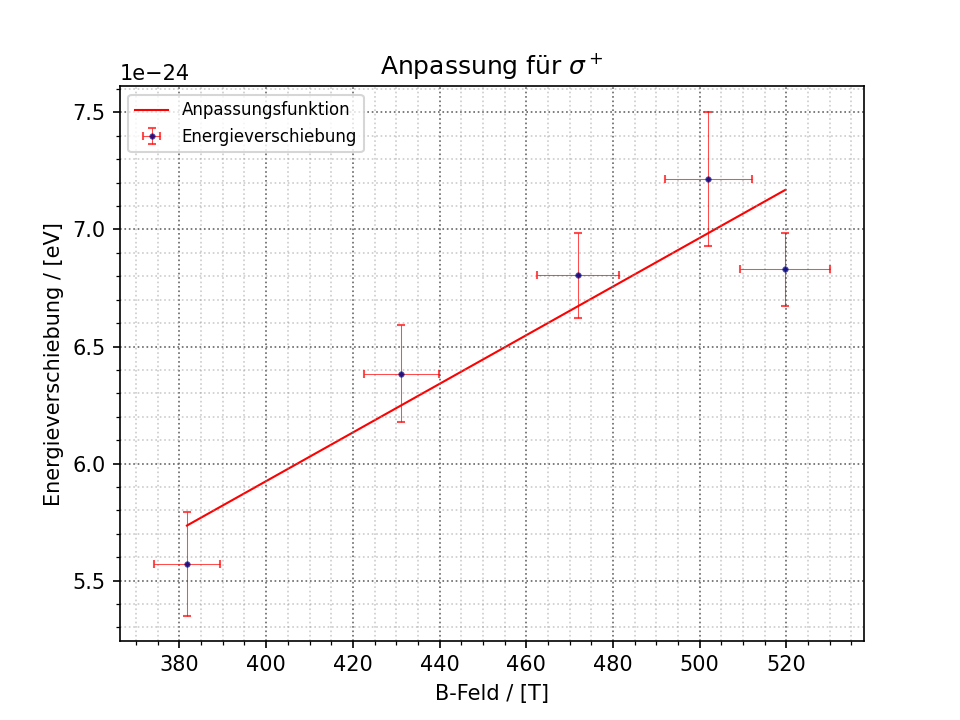
\includegraphics[width=.49\textwidth]{plots/E_mu_sigmaplus.png}}
    \subcaptionbox{Energieverschiebung aus den Peakschwerpunkten der $\sigma^-$-Linie in Abhängigkeit der Magnetfeldstärke mit Anpassungsfunktion gemäß~\cref{equ:deltaE_fit}\label{fig:deltaE_minus}}{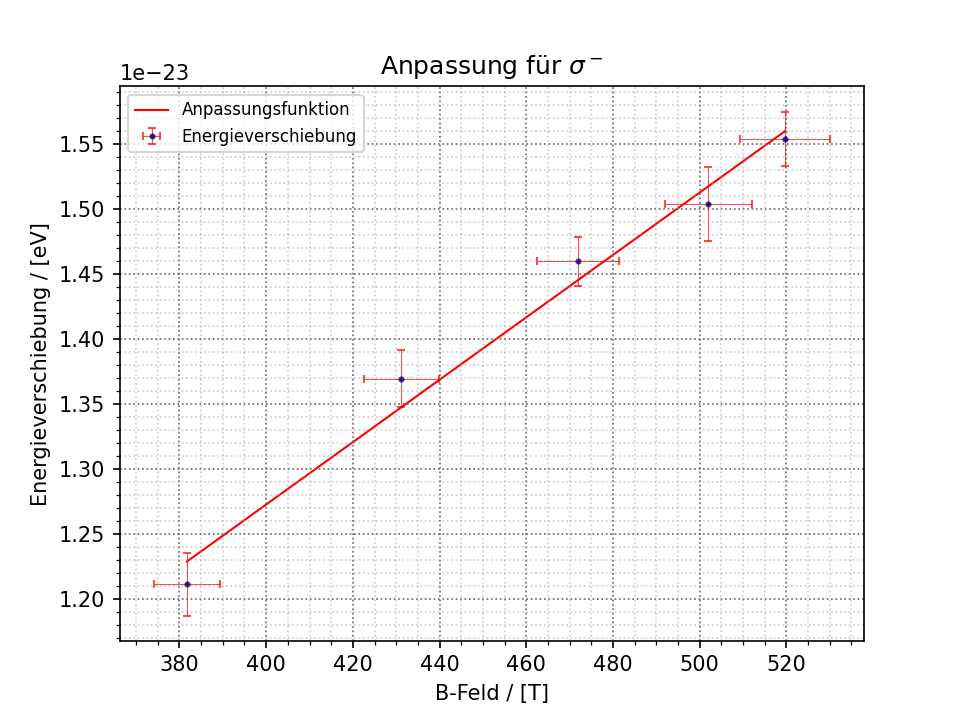
\includegraphics[width=.49\textwidth]{plots/E_mu_sigmaminus.png}}
\end{figure}

\noindent Die Anpassungsfunktionen (\cref{fig:deltaE_plus} und \cref{fig:deltaE_minus}) liefern folgende experimentelle Werte für das \texttt{Bohre}sche Magneton:
\begin{align}
    \mu_+ &= (\num{9.73e-24}\pm\num{1.61e-12}) \si{\joule\per\tesla} \\
    \mu_- &= (\num{24.43e-24}\pm\num{1.36e-12}) \si{\joule\per\tesla}
\end{align}
mit dem Varianzgewichteten Mittel:
\begin{equation*}
    \mu_{B,\text{exp}} = (\num{1.828e-23}\pm\num{1.472e-12})\si{\joule\per\tesla} 
\end{equation*}
Der Literaturwert~\cite{NIST} beträgt:
\begin{equation*}
    \mu_{B,\text{lit}} = \SI{9.2740100783(29)e-24}{\joule\per\tesla}
\end{equation*}
Der experimentell bestimmte Wert weicht stark vom Literaturwert ab und hat einen 12 Größenordnungen größeren Fehler.\\
Während der unpassende Fehler durch Fehlerhafte Auswertung zustande gekommen sein könnte (es besteht der starke Verdacht, dass irgendwo Einheiten verwechselt wurden) hat die starke Abweichung durch die Natur des Versuchs mehrere Fehlerquellen.
\vspace{0.2cm}
Die Kalibration des Magnetfeld könnte (abgesehen nicht ausreichend vieler Messdaten) verfälscht werden, wenn die Hall-Sonde nicht an der gleichen Stelle zwischen den Polschuhen befand\footnote{Wobei diese Begründung ausgeschlossen wird, da die beiden Kalibrationskurven gut miteinander übereinstimmten.}\\
Außerdem könnte es durch nicht exakt planparalleler Ausrichtung der optischen Bauteile zu Verzerrung kommen, sodass die Position der beobachteten Linien verschoben werden würden.
\vspace{0.2cm}
Die anschließende Modellierung der Peakschwerpunkte durch drei Gauss-Kurven entsprach auch nicht mit hinreichender Genauigkeit den Messwerte, was durch die $\chi_{\text{red}}^2$-Werte (siehe~\cref{tab:langzeeman-fit}) zu erkennen ist. Auch werden die Aufgenommenen Datenpunkte nicht gemittelt, weswegen von einer Momentanaufnahme der Spektrallinien mit entsprechenden Werten ausgegangen wird.
%
%--
%
\section{Weitergehende Überlegung}
Im folgenden werden noch das Auflösungsvermögen sowie die Finesse des \texttt{Fabry-Pérot}-Etalons und die Doppler-Verbreiterung der Linien abgeschätzt.
\subsection{Auflösungsvermögen und Finesse}
Die Finesse $\mathcal{F}$ ist ein Maß für das spektrale Auflösungsvermögen und definiert durch:
\begin{equation*}
    \mathcal{F} = \frac{\Delta \lambda}{\delta \lambda}
\end{equation*}
Hierbei ist $\Delta \lambda$ durch den freien Spektralbereich und $\delta \lambda$ durch die Halbwertsbreite (Transmissionskoeffizient $T = \SI{0.5}{}$) gegeben. Ersteres beschreibt die Wellenlängendifferenz zwischen zwei Wellenlängen, die bei Einfall komplett transmittiert werden (Transmissionskoeffizient $T = \SI{1}{}$) 
\vspace{0,2cm}
Das Auflösungsvermögen $A$ ist ein Maß dafür, wie gut zwei verschiedene, nebeneinanderliegende Wellenlängen noch getrennt wahrgenommen werden können:
\begin{equation*}
    A = \frac{\lambda}{\Delta \lambda}
\end{equation*}
Hier ist $\Delta \lambda$ (anders als bei der Finesse) die Wellenlängendifferenz, bei der man beide Linien noch getrennt beobachten kann. Mit gegebenen Daten des Etalons~\cite{praktikum4} können die zu erwarteten Größen bestimmt werden zu:
\begin{align*}
    \mathcal{F}&= \frac{\pi\sqrt{R}}{1-R} \approx 19\\
    A &= \frac{2nd\mathcal{F}}{\lambda_{\pi}^0} \approx 35\cdot10^4
\end{align*}
\newpage
\noindent Nun werden die experimentellen Messdaten verwendet werden um die daraus berechnete Finesse und Auflösungsvermögen zu vergleichen:
\begin{itemize}
    \item In der \textbf{transversalen Konfiguration} wurden die drei einzelnen Ringe bis zu einem Strom von $I = \SI{4.7\pm 0.2}{\ampere}$ aufgelöst. Über die Magnetfeldkalibrierung berechnet sich $B = \SI{307.2\pm 6.1}{\milli\tesla}$. Nun kann durch due geringe Wellenlängendifferenz zwischen den gerade noch getrennt wahrnehmbaren Linien die Näherung $E \approx \frac{hc}{\lambda_{\pi}^0}$ mit $\Delta E = \mu_B B$ (für benachbarte Linien gilt $\Delta M = 1$) und erhält:
        \begin{align*}
            A &\approx \frac{\lambda_{\pi}^0}{\Delta \lambda} 
                = \frac{\lambda_{\pi}^0}{\Delta \left(\frac{hc}{E}\right)}
                =  \frac{\lambda_{\pi}^0}{\frac{hc}{E^2}\Delta E}
                = \frac{hc}{\lambda_{\pi}^0\mu_B B} = \num{4.77e25} \pm 9.28\\
            \mathcal{F} &= \frac{\lambda_{\pi}^0 A}{2nd} = \num{2.64e21} \pm \num{5.12e-4}
        \end{align*}
    \item Für die \textbf{longitudinale Konfiguration} wird analog vorgegangen. Es wurde ein Strom $I = \SI{1.7\pm 0.2}{\ampere}$ aufgezeichnet, woraus die magn. Flussdichte $B = \SI{111.7\pm 2.2}{\milli\tesla}$ ermittelt wird. Es folgt die analoge Berechnung:
        \begin{align*}
            A &\approx \frac{hc}{2\lambda_{\pi}^0\mu_B B} = \num{13.12e25} \pm \num{25.52}\\
            \mathcal{F} &= \frac{\lambda_{\pi}^0 A}{2nd} = \num{7.25e21} \pm \num{1.41e-3}
        \end{align*}
    Der Faktor 2 im Nenner des Auflösungsvermögen kommt durch die Energiedifferenz, da die $\sigma^{\pm}$-Komponente energetisch doppelt so weit voneinander entfernt sind, als die $\pi$-Komponente.
    \item Ein Ausschnitt von zwei lokalen Maxima wird mit der CCD Kamera ohne Magnetfeld aufgenommen. Dafür wird an die Messwerte eine Summe von zwei \texttt{Gauss}-Kurven mit linearem Untergrund angepasst. Da hier nur die Position der Maxima sowie deren Halbwertsbreite benötigt genügt die genannte Anpassungsfunktion (\cref{fig:finesse}). Es folgen die Anpassungsparameter zu:
    \begin{align*}
        \mu_1 &= \SI{1.01740\pm 0.00038}{\degree} & \sigma_1 &= \SI{0.02534 \pm 0.00036}{\degree}\\
        \mu_2 &= \SI{1.29334\pm 0.00042}{\degree} & \sigma_2 &= \SI{0.02864 \pm 0.00042}{\degree}
    \end{align*}
    Für kleine $\alpha\approx 0$ folgt aus~\cref{equ:lambda}
    \begin{equation*}
        \lambda \approx \frac{2nd}{m}\left( 1- \frac{\sin^2(\alpha)}{2n^2} \right)
            \approx \frac{2nd}{m}\left( 1-\frac{\alpha^2}{2n^2} \right)
    \end{equation*}
    Da zudem $\mu_1\approx\mu_2\approx 0$ und $k\gg1$ kann die oben genannte Näherung angewendet werden, wodurch sich der freie Spektralbereich umformt zu:
    \begin{equation*}
        \Delta\lambda = \lambda_2-\lambda_1\approx\frac{d}{nk}(\mu_2-\mu_1)
    \end{equation*} 
    Die Halbwertsbreite einer \texttt{Gauss}-Funktion ist gegeben als das ($2\sqrt{2\log(2)}$)-Fache der Standardabweichung und es folgt:
    \begin{equation*}
        \delta\lambda\approx \frac{d}{nk}2\sqrt{2\log(2)}\sigma
    \end{equation*}
    Hierbei wird $\sigma = \SI{0.02673 \pm 0.00027}{\degree}$ als varianzgewichtete Mittel von $\sigma_{1,2}$ ist (Winkel müssen in \texttt{rad} angegeben werden). Es folgt:
    \begin{align*}
        \mathcal{F} &\approx \frac{\mu_2-\mu_1}{2\sqrt{2\log(2)}\sigma} = \SI{4.383\pm 0.045}{}\\
        A &= \frac{2nd\mathcal{F}}{\lambda_{pi}^0} = \SI{7.94(82)e4}{}
    \end{align*}
\end{itemize}

\begin{figure}[ht]
    \centering
    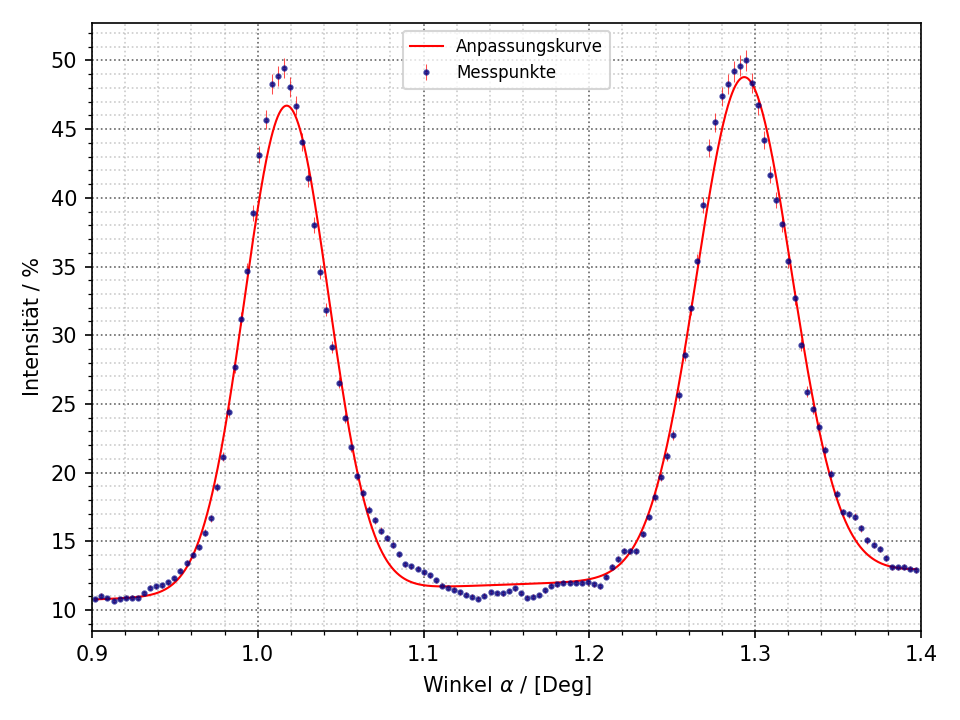
\includegraphics[width=.7\linewidth]{plots/finesse.png}
    \caption{Ausschnitt aus einem mit der CCDD-Kamera aufgenommenen Interferenzmusters ohne externes Magnetfeld}\label{fig:finesse}   
\end{figure}

\noindent Vergleicht man nun die drei experimentell bestimmten Werte mit dem theoretischen Wert sieht man, dass sich allein die letzte Methode zumindest in der richtigen Größenordnung befindet, wenn auch der theoretische Wert beinahe $\num{4.5}$-mal so groß ist. Die Werte aus der longitudinalen und transversalen Konfiguration bestätigt die Vermutung, dass hier ein Auswertungsfehler vorliegt, jedoch konnte der Fehler nach ausgiebigem Suchen und probieren nicht gefunden werden. Ein weiterer möglicher Einflussfaktor auf die ermittelten Werte ist die Breite $\sigma$ der verwendeten Anpassungsfunktion. Diese kann durch externe Effekte vergrößert sein, was zu einer Verfälschung der Ergebnisse führt. Zu den Ursachen zählen unter anderem die natürliche Linienbreite, die sich aus der endlichen Lebensdauer angeregter Zustände ergibt, sowie die Dopplerverbreiterung infolge der thermischen Bewegung der emmittierenden Atome. Eine genauere Betrachtung dieses Effekts wird im nachfolgenden Abschnitt behandelt.
%--
\clearpage
\subsection{Doppler-Verbreiterung der Linien}
Aufgrund der thermischen Bewegung der Teilchen wird die natürliche Linienbreite aufgrund des \texttt{Doppler}-Effektes vergrößert. Im Ruhesystem eines Cd-Atoms strahlt es (ohne externes Magnetfeld) mit der Wellenlänge $\lambda_{\pi}^0$. Bewegt es sich, wird diese Wellenlänge, so wird diese Wellenlänge gemäß des \texttt{Doppler}-Effekts vergrößert (Bewegung vom Beobachter weg) bzw. verkleinert (Bewegung auf den Beobachter zu). Mit der Annahme aus \cite{praktikum4}, dass die Cd-Lampe eine Temperatur von $T = \SI{1000}{\kelvin}$ hat, kann die Halbwertsbreite der Dopplerverbreiterung~\cite{Spektrum} für Cadmium mit einer Masse $m = \SI{112,4}{\mole}$\cite{CIAAW} wie folgt abgeschätzt werden:
\begin{equation*}
    \delta \lambda = \frac{\lambda_{\pi}^0}{c}\sqrt{\frac{8k_B T \log(2)}{m}} = \SI{1.4e-12}{\meter}
\end{equation*}
Da die angegebene Temperatur als grobe Schätzung der Größenordnung fungiert wird das Ergebnis ohne Fehler dargestellt. Im Vergleich zu dem mit der \texttt{CCD}-Kamera abgeschätztem Wert
\begin{equation*}
    \frac{\lambda_{\pi}^0}{A} \approx \SI{8.11e-12}{}
\end{equation*}
Hieraus folgt, dass die durch das Etalon mit bestimmten Auflösungsvermögen $A$ minimal auflösbare Verbreiterung fast 6-mal so groß ist, wie die Dopplerverbreiterung und diese aus deshalb nicht aufgelöst werden kann.